\documentclass{beamer}

\usepackage{txfonts}
\usepackage{hyperref}
\usepackage{fancybox}
\usepackage{xfrac}
\usepackage{cancel}


\newcommand{\heart}{\ensuremath\heartsuit}

\usepackage{mathtools,amssymb}
\newcommand{\myarrow}{\scalebox{2}[2]{$\mathclap{\curvearrowleft}\mkern2.2mu
                                                 \mathclap{\curvearrowright}$}}

\DeclareMathOperator{\Bin}{\mathrm{Bin}}

\hypersetup{colorlinks=false,linkbordercolor=red,linkcolor=green,pdfborderstyle={/S/U/W 1}}

\addtobeamertemplate{navigation symbols}{}{ \hspace{1em}    \usebeamerfont{footline}%
    \insertframenumber / \inserttotalframenumber}

\geometry{papersize={15cm,12cm}}
\usepackage{lipsum}

\makeatletter
\newenvironment<>{contdproof}[1][\proofname]{%
    \par
    \def\insertproofname{#1\@addpunct{.}}%
    \usebeamertemplate{proof begin}#2}
  {\usebeamertemplate{proof end}}
\makeatother


\setbeamertemplate{theorems}[numbered]

\newtheorem*{nonumdefinition}{Definition}
\newtheorem*{nonumproblem}{Problem}
\newtheorem*{nonumlemma}{Lemma}
\newtheorem*{nonumtheorem}{Theorem}
\newtheorem*{nonumproof}{Proof}
\newtheorem*{nonumremark}{Remark}
\newtheorem*{answer}{Answer}
\newtheorem*{nonumremarks}{Remarks}
\newtheorem*{nonumexamples}{Examples}
\newtheorem*{nonumsolution}{Solution}
\newtheorem*{nonumexample}{Example}
\newtheorem*{nonumproposition}{Proposition}
\newtheorem{proposition}[theorem]{Proposition}



\theoremstyle{alphtheorem}
\newtheorem{alphtheorem}{Theorem}
\renewcommand{\thealphtheorem}{\Alph{alphtheorem}}
\renewcommand{\thesection}{\arabic{section}}



\usepackage{tikz}
\newcommand*\mycirc[1]{%
  \tikz[baseline=(C.base)]\node[draw,circle,inner sep=.7pt](C) {#1};\:
}

\newcommand\myheading[1]{%
  \par\bigskip
  {\color{blue}{\large #1}}\par\smallskip}

%\usetheme{Warsaw}
%\usetheme{Berkeley} %sample 1

\usetheme{Berlin} % sample 2
%\usetheme{AnnArbor} % sample 3

\let\otp\titlepage
\renewcommand{\titlepage}{\otp\addtocounter{framenumber}{-1}}

\title{Lecture 22: Point Estimation}
\author{}
\date{}

\begin{document}
\begin{frame}[plain]
\titlepage
\end{frame}

\begin{frame}
Today we start Chapter 6 and with it the statistics port of the course. We saw in Lecture 20 (Random Samples) that it frequently occurs that we know a probability distribution except for the value of a parameter. 

In fact we had  three examples

\myheading{1. {\it The Election Example}}
\begin{center}
\begin{tabular}{|c|}
\hline\\
Bin (1, ?)\\
\\
\hline
\end{tabular}
\end{center}
\end{frame}

\begin{frame}
\myheading{2. {\it The Computer Failure Time Example}}
\begin{center}
\begin{tabular}{|c|}
\hline\\
Exp (?)\\
\\
\hline
\end{tabular}
\end{center}

\myheading{3. {\it The Random Number Example}}
\begin{center}
\begin{tabular}{|c|}
\hline\\
U(0, ?)\\
\\
\hline
\end{tabular}
\end{center}

By convention the unknown parameter will be denoted ? So replace ? by $\theta$ in the three examples. 
So $\theta = p$ in example 1 and $\theta = \lambda$ in Example 2 and $\theta = B$ (so $U (0, B)$) in Example 3.
\end{frame}

\begin{frame}
If the population $X$ is discrete we will write its proof as $p_X (x,\theta)$ to emphasize that it depends on the unknown parameter $\theta$ and if $X$ is continuous we will write its pdf as $f_X (x, \theta)$ again to emphasize the dependence on $\theta$.

\myheading{{\it Important Remark}}
$\theta$ is a fixed number, it is just that we don't know it. But we are allowed to make calculations with a number we don't know, that is the point of known and ``the unknown $x$''.
\end{frame}

\begin{frame}
Now suppose we have on actual sample $x_1, x_2, \ldots, x_n$ from a population $X$ whose probability distribution is known except for an unknown parameter $\theta$. For convenience we will assume $X$ is discrete.

\medskip
\centerline{\includegraphics{figure/art22(1).eps}}

The idea of point estimation is to develop a theory of making a guess for $\theta$ (``estimating $\theta$'') in terms of $x_1, x_2, \ldots, x_n$.

So the big problem is 
\end{frame}

\begin{frame}
\myheading{The Main Problem (Vague Version)}

What function $h(x_1, x_2, \ldots, x_n)$ of the items $x_1, x_2, \ldots, x_n$ in the sample should we pick to estimate $\theta$ ?

\begin{nonumdefinition}
Any function $w= h(x_1, x_2, \ldots, x_n)$ we choose to estimate $\theta$ will he called an estimator $for$ $\theta$.

As first one might ask -
\begin{equation*}
\left. 
\begin{tabular}{ll}
find $h$ so that for every sample \\
$x_1, x_2, \ldots , x_n$ we have  \\
\qquad $h(x_1, x_2, \ldots, x_n) = \theta$.  
\end{tabular}
 \right\} \tag{$\ast$}\label{eq-*}
\end{equation*}

This is {\it hopelessly naive}. Let's try something else
\end{nonumdefinition}
\end{frame}

\begin{frame}
\myheading{{\it The Main Problem (some what more precise)}}

Give quantitative criteria to decide whether one estimator $w = h_1 (x_1, x_2, \ldots, x_n)$ for $\theta$ is better than another estimator $h_2 (x_1, x_2, \ldots, x_n)$.

The above version, though better, is still not useful. 

In order to pose the problem correctly we need to consider random samples from $X$, in ofter words go back before an actual sample is taken or ``go random''.
\end{frame}

\begin{frame}
\centerline{\includegraphics{figure/art22(2).eps}}
\smallskip

Now our {\it function $h$ gives rise to a random variable (statistic)}

$$
W = h (X_1, X_2, \ldots, X_n)
$$
which I will call (for a while) an estimator {\it statistic}, to distinguish if from the estimator ({\it number}) $w= h(x_1, x_2, \ldots, x_n)$. Once we have chosen $h$ the corresponding  estimator statistic will ofter be denoted $\hat{\theta}$.
\end{frame}

\begin{frame}
If we have an actual sample 

\medskip
\centerline{\includegraphics{figure/art22(1).eps}}
then the {\it number} $h(x_1, x_2, \ldots, x_n)$ is called the observed value of the estimator statistic $W = h (X_1, X_2, \ldots, X_n)$ on the sample $x_1, x_2,\ldots, x_n$. Unfortunately if too is after denoted $\hat{\theta}$.

\begin{nonumremark}
The estimator statistic should be denoted $\hat{\theta}$ and its observed value $\hat{\theta}$ but mathematical (and statistical) ?????? is for from consistent. 
\end{nonumremark}
\end{frame}

\begin{frame}
\myheading{Main Problem (third version)}

Find an estimator $h(x_1, x_n)$ so that
\begin{equation*}
P (h (x_1, X_2, \ldots, X_n) = \theta) \tag{$\ast\ast$}\label{eq-**}
\end{equation*}
is maximized 

This is what we want but it is too hard to implement - after all we don't know $\theta$.

\myheading{Important Remark}
We have made a huge gain by ``going random''. The statement ``maximize $P(h(x_1, x_n) =\theta)$'' is stupid, idiotic, foolish...
\end{frame}

\begin{frame}
because {\it $h(x_1, \ldots  x_n)$ is a number and $\theta$ is a number} so the above statement amounts to the hopelessly naive criterion from page 5

-choose $h$ so that $h(x_1, x_2, \ldots , x_n) = \theta$.

Now we weaken \eqref{eq-**} to something that can be achieved, in fact achieved surprising easily.
\end{frame}

\begin{frame}
\myheading{Unbiased Estimators Mam Problem (fourth version)}

Find an estimator $w = h (x_1,\ldots, x_n)$ so that the expected value $E(W)$ of the estimator statistic $W$ satisfies 
\begin{equation*}
E(W) = \theta \tag{$\ast\ast\ast$}\label{eq-***}
\end{equation*}

At first glance \eqref{eq-***} doesn't look much easier to achieve then \eqref{-**} but in fact it is surprising easy to achieve - in fact too easy. There are money $W$ that satisfy \eqref{eq-***} so we will need further criteria. 
\end{frame}

\begin{frame}
Let's give estimator statistics that satisfy \eqref{eq-***} a name.

\begin{nonumdefinition}
An estimator statistic 

$W = h(X_1, X_2, \ldots, X_n)$ is an {\it unbiased estimator} of the population parameter $\theta$ of 
$$
E(W) = \theta.
$$
\end{nonumdefinition}

Intuitively \eqref{eq-***} is a good idea but we can make this move precise Various theorems in probability e.g Cheston's requetity.
\end{frame}

\begin{frame}
tell us that if $Y$ is a random variable and $Y_1, Y_2, \ldots, Y_n$ are observed values of $Y$ then the numbers $y_1, y_2, \ldots, y_n$ will tend to be near $E(Y)$.

Applying this to our statistic $W$- if we take many samples of size $n$ and compute the value of our estimator $h$ on each one to obtain many observed values of $W$ then the resulting numbers will be near $E (W)$. But we want there to be near $\theta$. So we want 
$$
E(W) = \theta
$$
\end{frame}

\begin{frame}
\medskip
\centerline{\includegraphics{figure/art22(3).eps}}

I have run out of letters. In the above there are four sample of size $n$ and four corresponding estimates $h(w_1, \ldots, w_n)$, $h(x_1, \ldots, x_n)$, $h(y_1, \ldots, y_n)$ and $h(z_1, \ldots, z_n)$.

Imagine that instead of four we have one hundred estimates of size $n$ and one hundred estimates. Then if $E(W) = \theta$ most of these estimates would be close to $\theta$.
\end{frame}

\begin{frame}
{\it Examples of Unbiased Estimators The most important estimation problem}

Let's take another look at Problems 1 and 2 (pages 1 and 2)

%\figure

%\figure

\begin{tabular}{ll}
Facts - & for a Bernoulli random \\
& variable $X \sim \Bin (1, p)$ \\
& we have $E(X)=p$\\
& {\it and}\\
& for an exponential  random \\
& variable $X \sim \text{ Exp } (\lambda)$
\end{tabular}
$$
E(X) = \lambda
$$
\end{frame}

\begin{frame}
\myheading{So in both cases the unknown parameter is the population mean $E(X) = \mu$}

We have 

\begin{nonumproblem}
Find an unbiased estimator for the population mean $\mu$

\medskip
\centerline{\includegraphics{figure/art22(4).eps}}

So we wont $h(x_1, x_2, \ldots, x_n)$ so that
$$
E\left( h \left( X_1, X_2, \ldots, X_n\right) \right) = \mu
$$
= the {\it population} mean.
\end{nonumproblem}
\end{frame}

\begin{frame}
  Amazingly there is a very simple solution to the no matter what the underlying distribution is

\begin{nonumtheorem}
The sample mean $\bar{X}$ is an unbiased estimator of the population mean $\mu$; that is 
$$
E(\bar{X}) = \mu
$$
\end{nonumtheorem}

\begin{nonumproof}
The proof is so simple, deceptively simple because the theorem is so important.
\begin{align*}
E(\overline{X}) & = E \left(\frac{X_1 + \ldots + X_n}{n} \right)\\
& = \frac{1}{n} \left(E(X_1) + \ldots + E (X_n) \right)
\end{align*}
\end{nonumproof}
\end{frame}

\begin{frame}
\begin{proof}[Proof (Cont.)]
But $E(X_1) = E (X_2) = \ldots = E (X_n) = \mu$
because all the $X_1$'s are samples from the population so they have the same distribution as the population so
\begin{align*}
E(\overline{X}) & = \frac{1}{n} \left(\mu + \mu + \ldots \mu \right)\\[-0.43cm]
&  \qquad \quad\underbrace{\qquad \qquad ~~~~}_{n \text{ times}}\\
& = \frac{1}{n} (n, \mu)\\
& = \mu
\end{align*}
\end{proof}
\end{frame}

\begin{frame}
For the problem of estimating $P$ in $\Bin(1,p)$ we have 
$$
\overline{X} = \frac{\text{number of observed successes}}{n}
$$

Since each of $x_1, x_2, \ldots, x_n$ is either 1 on 0 so
$$
x_1 + x_2 + \ldots + x_n = \# \text{ of } 1's.
$$
Thus $\overline{x}$ is the ``common sense'' estimator, the relative number of observed successes.
\end{frame}

\begin{frame}
\myheading{An Examples Where the ``Common Sense'' Estimator is Biased}

Once we have a {\it mathematical} criterion for an estimator to be good we will often find to our surprise that ``common sense'' estimators do not meet this criterion. We saw an example of this in the ``Pandemonium jet fighter'' problem 14, on page 242.

Another very similar problem occurs in Example 3 - estimator $B$ in choosing a random number from $U (0, B)$.
\end{frame}

\begin{frame}
\medskip
\centerline{\includegraphics{figure/art22(5).eps}}

The ``common sense'' estimator for $B$ is $w = \text{ max } (x_1, x_2, \ldots, x_n)$, the biggest number you observe. But it is intuitively clear that this estimate will be too small since it only gives the right object if one of the $x$'s is equal to $B$ and
\begin{gather*}
P\left(\bigcup\limits^n_{1=1} (X_1 = B)\right) = \sum\limits^n_{1=1} P(X_1  = B)\\
= 0 + 0+\ldots + 0 =0
\end{gather*}
\end{frame}

\begin{frame}
So the common sense estimator $W = \text{ max} (x_1, x_2, \ldots, x_n)$ is biased.
$$
E \left( \text{Max }\left(X_1, \ldots, X_n\right) \right) \displaystyle{\mathop{<}_{\neq}} B 
$$

Amazingly, if you do page 252, problem 32 {\it you will see exactly by how much if undershoots the mark}.

\begin{nonumtheorem}
$$
E \left(\text{Max} (X_1, X_2, \ldots, X_n) \right) = \dfrac{n}{n+1} B
$$ 
so $\left(\dfrac{n+1}{n} \right) \text{ Max } (X_1, X_2, \ldots, X_n) $ is unbiased.
\end{nonumtheorem}

{\it Mathematics trumps common sense}
\end{frame}

\begin{frame}
\myheading{Minimum Variance Unbiased Estimators}

We have seen that $\overline{X}$ and $X_1$ are unbiased estimators of the population mean. Common sense tells us that $\overline{X}$ is 
better.

What mathematical criterion separates  them. We have 
\begin{align*}
V (X_1)  & = \sigma^2 = \text{ the population variance}\\
V (\overline{X}) & = \frac{\sigma^2}{n}
\end{align*}
so 
$$
V (\overline{X}) \text{ is a lot smaller than } V(X_1).
$$
\end{frame}

\begin{frame}
We will see later why this is good. First we state 

\myheading{The Principle of Minimum Variance Unbiased Estimation}

Among all estimators of $\theta$ that are unbiased, choose one that has minimum variance.

The resulting estimator is called a minimum variance unbiased estimator, MVUB.
\end{frame}

\begin{frame}
\begin{theorem}
$\overline{X}$ is a minimum variance unbiased estimator for the problems of 
\begin{itemize}
\item[1.] Estimating $p$ in Bin $(1,p)$

\item[2.] Estimating $\mu$ in $N(\mu, \sigma^2)$
\end{itemize}
\end{theorem}

Why is it good to minimize the variance?

The following is treated incompletely on page 252, \#34.
\end{frame}

\begin{frame}
Suppose $\hat{\theta} = h (X_1, X_2, \ldots, X_n)$ is an estimator statistic for an unknown parameter $\theta$.

\begin{nonumdefinition}
The mean squared error $MSE (\hat{\theta})$ of the estimator $\hat{\theta}$ is defined by 
$$
MSE (\hat{\theta}) = E \left((\hat{\theta} - \theta)^2 \right)
$$
so 
\begin{align*}
MSE (\hat{\theta}) & = \int \ldots \int\limits_{\mathbb{R}^n} (h(x_1, \ldots, x_n) - \theta)^2 f_{X_1} (x_1) \ldots f_{X_n} (X_n) dx_1, dx_2, \ldots , d_{X_n}.\\
\text{or } & = \sum\limits_{\text{all } x_1, x_n}\left( h(x_1, \ldots, x_n) - \theta\right)^2 P(X_1 = x_1) \ldots P(X_n = x_n)
\end{align*}
\end{nonumdefinition}
\end{frame}

\begin{frame}
So $MSE (\hat{\theta})$ is the squared error $(h(x_1, x_n) - \theta)^2$ of the estimate of $\theta$ by $h(x_1, x_2, \ldots, x_n)$ averaged over all $x_1, x_2, \ldots, x_n$.

Obviously we wont to minimize this squared error. Here is the point.

\begin{nonumtheorem}
If $\hat{\theta}$ is unbiased then
$$
MSE (\hat{\theta}) = V (\hat{\theta})
$$

This is amazingly easy to prove.
\end{nonumtheorem}
\end{frame}

\begin{frame}
\begin{proof}
If $\hat{\theta}$ is unbiased then $E (\hat{\theta}) = \theta$ so
$$
MSE (\hat{\theta}) = E \left( (\hat{\theta} - E (\theta)^2)\right)
$$
By definition the RHS is $V (\hat{\theta})$.
\end{proof}

Here is on important definition used a lot in the text.

\begin{nonumdefinition}[text page 238]
The standard error of the estimator $\hat{\theta}$, denoted $\sigma_{\hat{\theta}}$ is $\sqrt{V (\hat{\theta})}$. 

It is of the denoted $s_{\hat{\theta}}$ (not quite true) see page 238.
\end{nonumdefinition}
\end{frame}
\end{document}



